\documentclass{llncs}
\usepackage{amsmath,amssymb,algorithm,algorithmic}
\usepackage{hyperref,color}
% No page numbers.
\usepackage{subfig}
\usepackage{graphicx}

\newcommand{\tool}{\text{ANTsR}}
\newcommand{\R}{{\bf R}}
\newcommand{\X}{{\bf X}}
\newcommand{\Xh}{{\hat{{\bf X}}}}
\newcommand{\x}{{\bf x}}
\newcommand{\Y}{{\bf Y}}
% \newcommand{\U}{{\bf U}}
\newcommand{\V}{{\bf V}}
\newcommand{\E}{{\bf E}}
\newcommand{\y}{{\bf y}}
\newcommand{\Z}{{\bf Z}}
\newcommand{\z}{{\bf z}}
\newcommand{\bSigma}{\boldsymbol \Sigma}
\newcommand{\vect}[1]{\mathbf{#1}}
\newcommand{\field}[1]{\mathbf{#1}}
\newcommand{\image}[1]{#1}
\newcommand{\I}{\image{I}}
\newcommand{\J}{\image{J}}
\renewcommand{\u}{\vect{u}}
\renewcommand{\v}{\vect{v}}
\renewcommand{\c}{\vect{c}}
\newcommand{\h}{\vect{h}}
\newcommand{\w}{\vect{w}}
\newcommand{\myphi}{\phi}
\newcommand{\mypsi}{\psi}
\newcommand{\D}{D}
\renewcommand{\d}{\nabla}
\newcommand{\dd}{\text{d}}
\newcommand{\p}{\partial}
\renewcommand{\L}{\Delta} % laplacian
\newcommand{\myS}{S}
\newcommand{\myR}{R}
\newcommand{\myE}{E}
\newcommand{\ld}{\langle}
\newcommand{\rd}{\rangle}
\newcommand{\LL}{\mathcal{L}} % operator L
\newcommand{\tQ}{\mathcal{Q}}
\newcommand{\Id}{\text{Id}}
\newcommand{\tG}{{G}} % operator L
\newcommand{\Diff}{\text{Diff}}
\newcommand{\VV}{\mathcal{V}}
\newcommand{\opL}{\mathcal{L}}
\newcommand{\bs}{\boldsymbol}
\newcommand{\tk}{~ITK$^{\text{4}}$~}
\newcommand{\bsp}{$\substack{
   \rightsquigarrow \\
   b
  }$}
\newcommand{\mi}{$\substack{
   \approx \\
   \text{mi}
  }$}
\newcommand{\cc}{$\substack{
   \approx \\
   \text{cc}
  }$}
\usepackage{setspace,verbatim}
\begin{document}
\vspace{-0.1in}
\title{Standardized Registration Methods for the SATA Challenge Datasets}
\author{Brian B. Avants$^1$, Nicholas J. Tustison$^2$, Hongzhi
  Wang$^1$, Andrew J. Asman$^3$ \\and the
  $^5$\href{http://www.insightsoftwareconsortium.org/}{Insight
    Software Consortium}}
\institute{$^1$Penn Image Computing and Science Lab \\ Dept. of Radiology \\University of
  Pennsylvania, Philadelphia, PA, 19104\\ 
  $^2$Dept. of Radiology and Medical Imaging, \\ University of Virginia,
  Charlottesville, VA 22903\\
Electrical Engineering, Vanderbilt University, Nashville, TN, USA 37235\\
 $^5$\href{http://www.insightsoftwareconsortium.org/}{http://www.insightsoftwareconsortium.org/}}
\maketitle              
\begin{abstract}
The 2012 Segmentation: Algorithms, Theory and Applications (SATA)
challenge suggests that even subtle variation in registration
performance may impact the outcome of multi-atlas segmentation
algorithms. The 2013 SATA challenge organizers therefore requested
standardized registration that enables entrants to use the same
mappings as input to competing algorithms.  We therefore collaborated
to provide, within a relatively brief window of time, over 22,000
registration results based on Advanced Normalization Tools
(\url{http://stnava.github.io/ANTs/}).
The diencephalon component of the challenge presented familiar and
easily addressed data requiring only 1,600 mappings between different
3D human T1 neuroimages.  The 3D multiple modality MRI ``dog leg'' dataset ($>$ 7,000
mappings) presented the opportunity to improve performance by using
a multivariate similarity metric.  The 4D cardiac (or CAP) dataset
($\approx$ 13,000 mappings) includes highly variable image quality, anatomy
and field of view.  We detail the ANTs variants that address the most basic brain dataset, where we used
a template-based approach, to the more challenging CAP dataset which
employed a more customized registration solution based on prior
knowledge.  The scripts, source code and a small set of example data
accompany this paper and are available online.  
\footnote{This work is supported by National Library of Medicine sponsored ARRA stimulus
funding. Resources for this report are here \href{https://github.com/stnava/KnobSock}{(link)}.}
\end{abstract}

\begin{comment}
Brian,
 
One of the results of our multi-atlas workshop / challenge was that registration often had a larger impact on method performance than the statistical combination method (no real surprise there: garbage in = garbage out). SyN was used by the top two groups using Arno Klein’s published parameters.
 
In our journal write-up of the workshop results, we are planning on re-running the fusion algorithms using a common registration. Would you be willing to provide the “definitive” SyN results? We have 15 source images (plus label maps) that we need to match pair-wise to 20 target images (without label maps). If you would prefer to specify the command line parameters, Andrew (cc’d) can run the data through on our system.
 
Thanks!
Bennett

Dr. Avants,

After last year's MICCAI whole-brain segmentation challenge, two things became abundantly clear: (1) in order to isolate the benefits of specific label fusion algorithms we need to have a standardized registration and (2) the ANTs registration package represents the premier image registration framework. 

As a result, for this year's challenge (as part of the SATA workshop ) we would like to provide standardized atlas-target registrations for each of the datasets that we are considering.

Would you be willing to contribute these standardized registrations for the challenge?

The workshop website can be found here:
https://masi.vuse.vanderbilt.edu/workshop2013/index.php/Main_Page

The information on each of the datasets can be found here:
https://masi.vuse.vanderbilt.edu/workshop2013/index.php/Segmentation_Challenge_Details

The complete data package can be downloaded here:
https://masi.vuse.vanderbilt.edu/workshop2013/index.php/SATA_Data_Registration_Form

 For this year's challenge we are considering 3 datasets:
(1) A diencephalon (mid-brain) dataset
(2) A canine leg dataset
(3) A cardiac atlas dataset

 ``From my perspective, I think that the mid-brain and canine leg
  datasets would not be terribly difficult to achieve consistent
  correspondence across the images. However, the cardiac atlas dataset
  might be significantly more challenging due to the way in which the
  images are acquired (i.e.,wildly varying orientations and
  fields-of-view).'' ---{\em SATA Organizers}

We would greatly appreciate your help for making this challenge as successful as possible. If you have any questions/comments/concerns please do not hesitate to bring them up.

Thanks again,
Andrew Asman

\end{comment}

\section{Introduction}
Several early papers in image registration / segmentation focus on 
clinical applications including microscopy, nuclear medicine, tracking longitudinal
change and angiography
\cite{Badran1991,Venot1986,Venot1984,Wrigley1982,Adair1981}.  Rapid progress in registration
theory and implementation followed these early developments with
focus, in general, on either similarity metrics \cite{Wells1996},
transformation models \cite{Miller2005} or the combination of these in a general
purpose method \cite{Rueckert1999}.  More recently, as the core technology of segmentation and
registration mature, the research focus has returned to specific clinical
applications such as radiation therapy \cite{Chan2013}, drug discovery \cite{Fox2009},
neurosurgery \cite{Omara2013} and image-based biomarkers of pain \cite{Loggia2013}.  
Quantitative image mapping is also relied upon heavily for automated analysis of large datasets
such as ADNI \cite{Weiner2012} that cannot be processed ``by hand.''

These new problem domains are revealing the limitations of traditional
methods.  Brain registration methods, for instance, often assume that
a single reference space / template is adequate to combine information
across a population and that there exists, roughly, a diffeomorphism
between any pair of individual brains.  Segmentation methods, on the
other hand, often assume that intensity and object smoothness or
texture encode the shape to be segmented or that a single model object
is sufficient to act as a prior.  These assumptions may not
hold when imaging other organs or in emerging MR modalities.  

Multi-atlas segmentation and registration (MASR) methods help overcome
the limitations associated with mapping to a single template or using
a single exemplar segmentation.  These methods encode the notion that
different topology or image contrast may exist between different
subjects and, further, that the user cannot know these subjects {\em a
priori}.  In this case, the problem is to develop algorithms that
automatically adjust for registration accuracy at both global and
local scales and determine segmentation labels that incorporate
confidence.  MASR therefore enables applications that do not depend upon
successful pair-wise registration between all subjects, a goal that is
currently beyond the reach of any general purpose registration tool.

The organizers of the SATA 2013 challenge collected datasets that
frame, with specific examples, the issues raised above.  The
organizers wrote on May 10, 2013 ``in order to isolate the benefits of
specific label fusion algorithms we need to have a standardized
registration.''  The ANTs development team agreed to collaborate on a set of standard registration results for the challenge.  We
felt that our participation was important due to the variety of the challenge
data, the fact that not all entrants are biomedical image registration
experts and the results of SATA 2012 which suggested that a common
transformation basis set would help isolate the differences between
the segmentation component in MASR.  In other words, using a common
set of ``voters'' allows a more direct comparison of the
segmentation/fusion methods that are currently at the heart of the
SATA challenge. We present,
below, the ANTs techniques that address the unique hurdles as well as
opportunities afforded by this diverse collection of images.

\section{Methods} Three MRI datasets constitute the driving biological
problems for the 2013 challenge: T1-weighted whole head images of the
diencephalon (mid-brain), multi-modality T1 and T2 canine leg images
and a 4D cardiac atlas dataset.  The SATA organizers requested that we
provide transformed label sets and intensity images for all
training$\leftrightarrow$testing and training$\leftrightarrow$training
pairs.  The registration goal was to map the images with ``reasonable
and consistent'' performance and an open-source system.

We processed all data with Advanced Normalization Tools ( git commit
e3ba1c527fa63cc524bae7912b415d77adadc165 ) based on ITKv4.  The
processing was organized with a combination of bash or perl scripts
and run through standard Sun Grid Engine distributed computing.  The
core methods are available in ANTs programs \texttt{antsRegistration},
\texttt{ImageMath} (utilities), \texttt{N4BiasFieldCorrection} (bias
correction) and \texttt{Atropos} (segmentation).  These core tools are
described in archived publications
\cite{Tustison2010,Avants2011a,Avants2011}.  However, we employed
several new additions to ANTs registration that are as recent as 2013
and which are based upon our work for version 4 of the Insight
ToolKit.

\subsection{The (Fire) ANTs System} ANTs fundamentals involve pairwise
registration of images defined in physical space.  ANTs registrations,
as of 2013 with the Fire beta, are defined by an initial transformation (possibly the
identity) of the ``fixed'' and/or ``moving'' images.  This is followed
by a series of registration stages typically with increasing degrees
of freedom.  Each stage begins with $k$ similarity metric definitions
(most often $k=1$) and is followed by parameters defining the
multi-resolution strategy.  Subsequent stages may be added in the same
style.  Finally, ANTs takes options controlling optimization details
and pre/post-processing.  Application-specific choices should be made
for the transformation, similarity metrics and multi-resolution
strategy.  A variety of options are exercised in SATA processing.

\subsection{Diencephalon/Brain Data (SATA-B)}
 \begin{quote}
 ``... the mid-brain and canine leg
  datasets should not be terribly difficult ...'' ---{\em SATA Organizers}
\end{quote}
\begin{figure}[t]
 \centering 
  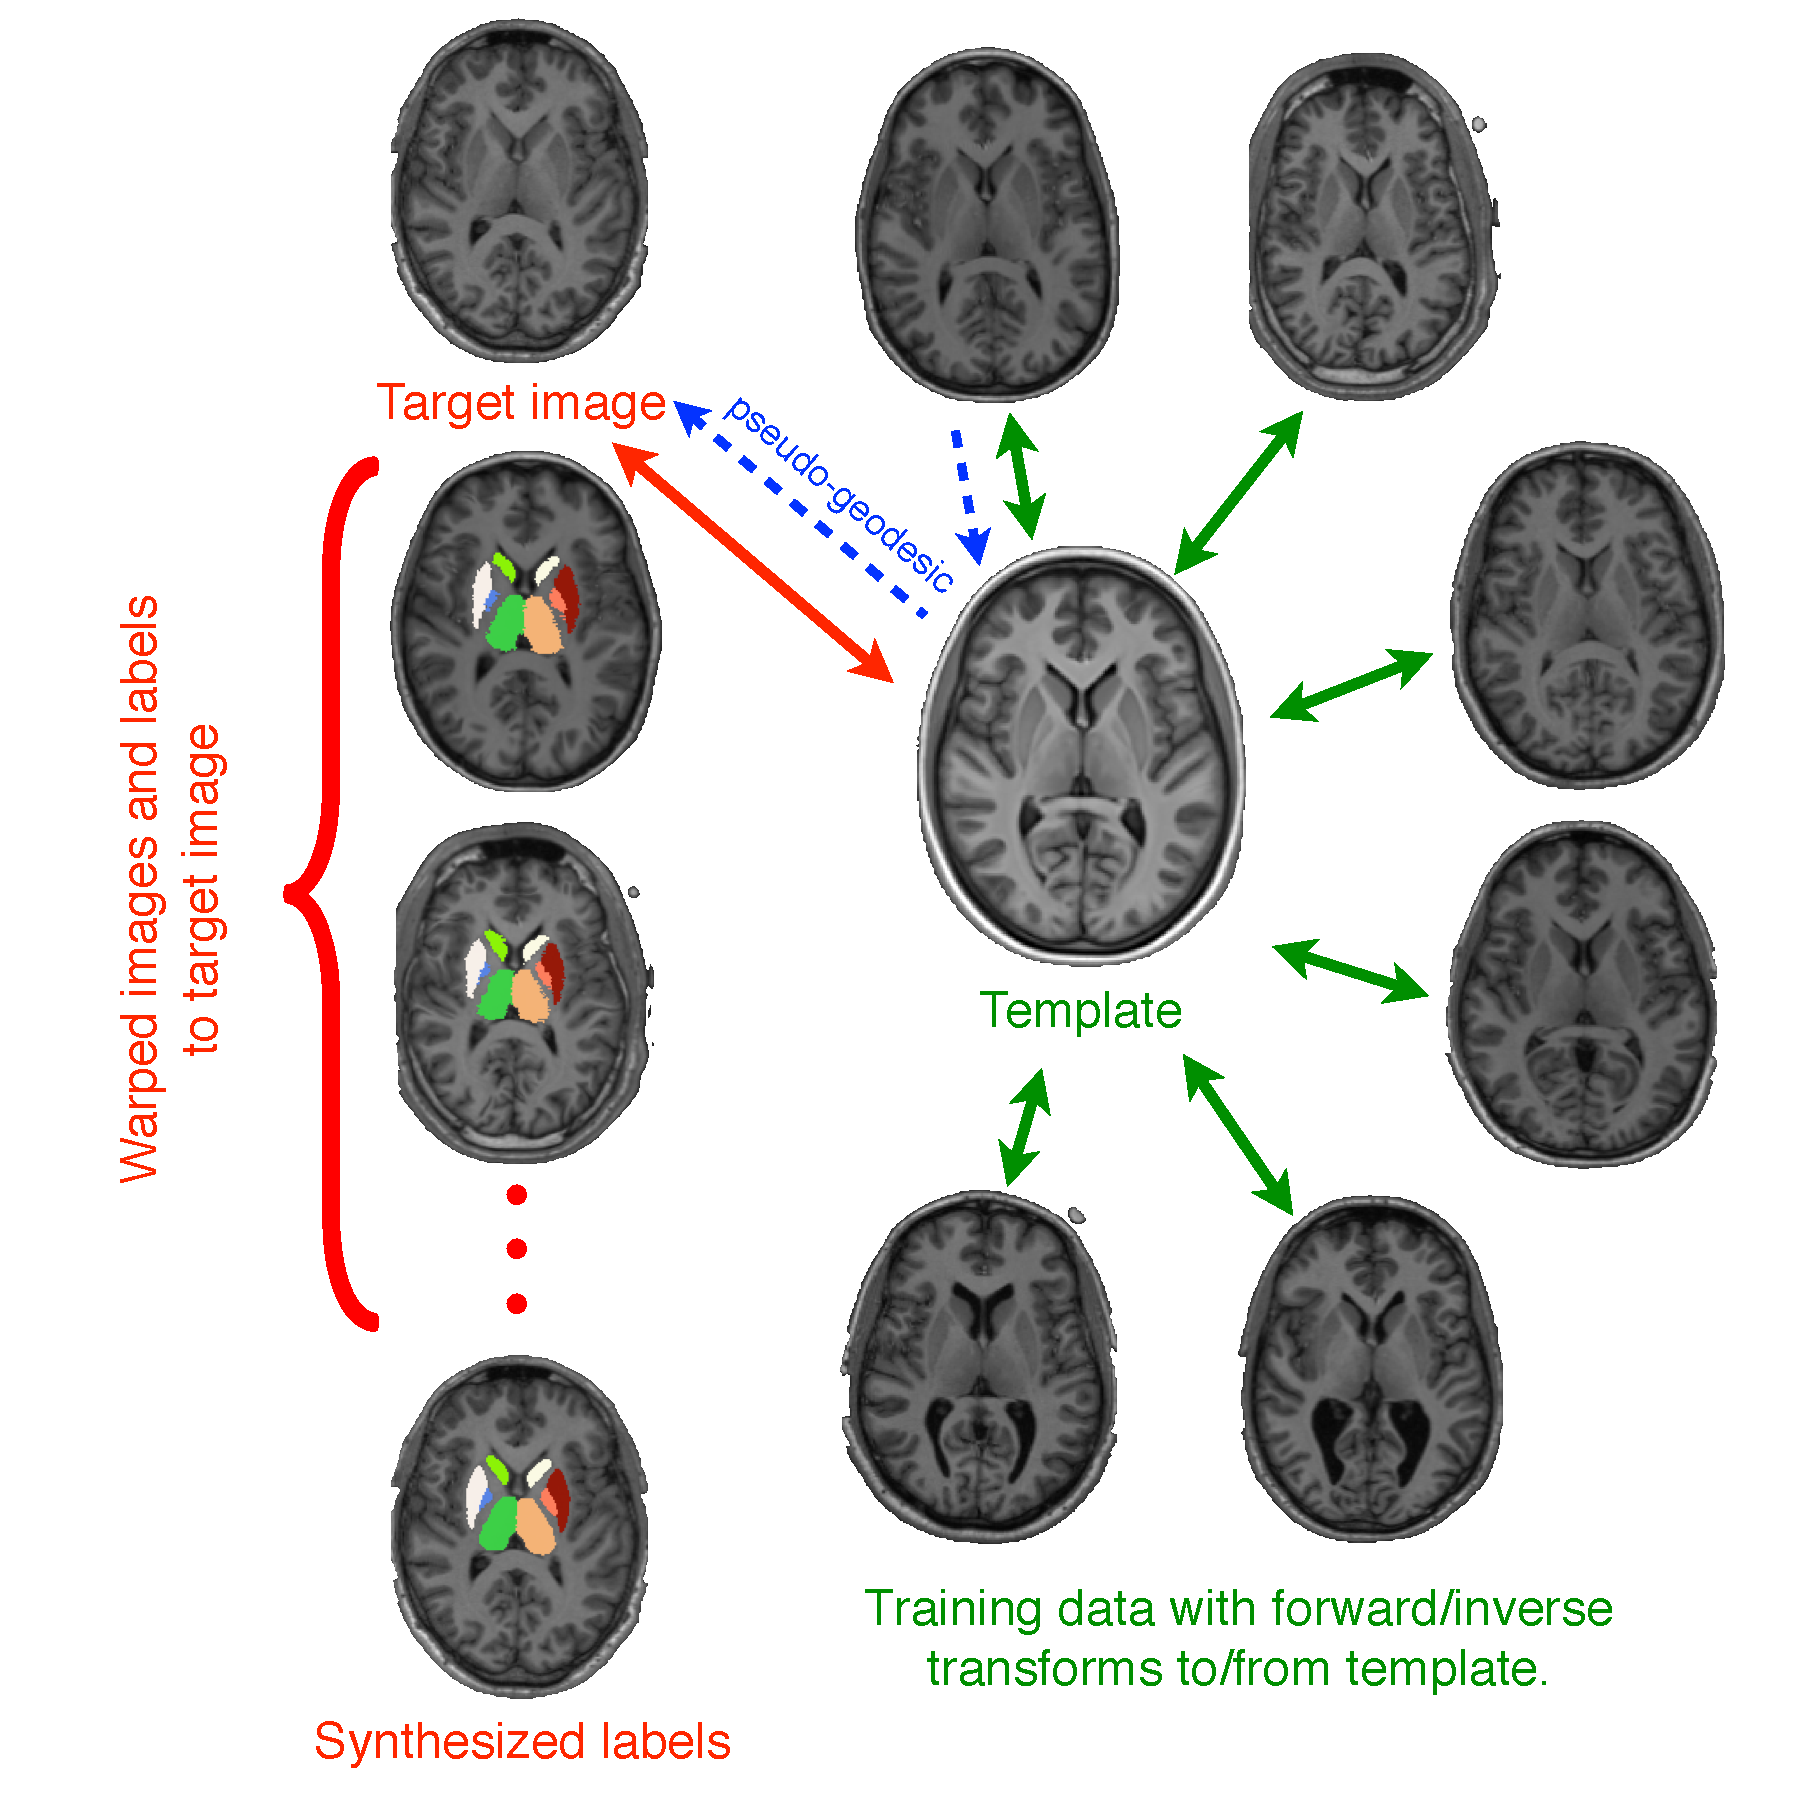
\includegraphics[width=3.5in]{../figs/SATA_diencephalon.pdf}
 \caption{SATA-B registrations map every image to every other image
   through the optimal template space (available online).  This
   requires only $n$ registrations rather than $n^2$.}
 \label{fig:Bmethods}
\end{figure}
We employed an efficient ``pseudo-geodesic'' processing strategy for this data to
avoid explicitly computing $\approx$1,600 image registration
instances, as shown in Figure~\ref{fig:Bmethods}.  As was shown in previous work (technical report), this
strategy improves upon single template labeling while approaching (not
equaling) the more computationally expensive all-pairs
registration required by standard MASR.

We first derive a custom whole-head template for this dataset and
extract the template cerebrum using MASR and LPBA40 labels \cite{Shattuck2008}.
We then extract the cerebrum from the individual SATA-B images based
on existing ANTs software (\texttt{extractBrainAllSubjects.pl}) for
template-based brain mapping.  We then re-registered the individual
cerebrum images to the template cerebrum
(\texttt{runSyNRegistrations.pl}).  The subject $n$ to template
mapping composes with the inverse of the subject $m$ to template
mapping to create the final mapping between subject $n$ and subject $m$.
The affine and deformable components of the SATA-B maps derive from
standard \texttt{antsRegistration} parameters.  The template is
available in the \texttt{data/SATA-B-Template/} directory.
 
\subsection{Dog Leg Multi-Modality Data (SATA-L)}
\begin{figure}[t]
 \centering 
  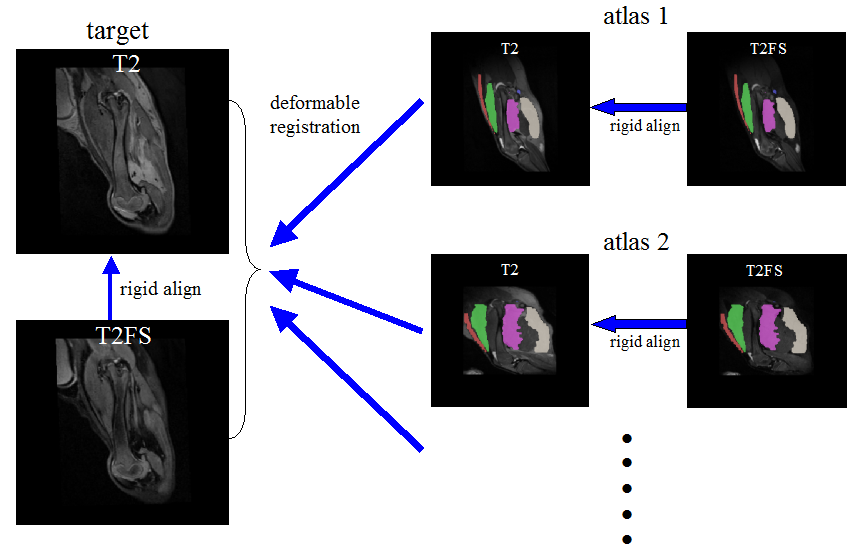
\includegraphics[width=3.5in]{../figs/canine-leg-registration.png}
 \caption{The SATA-L registration is similar to SATA-B.  However, the
image similarity is driven by the mutual information applied to both
modalities.  We chose to treat both modalities equally except for one
small detail---one of the modalities is rigidly registered,
intra-subject, to the other before proceeding with inter-subject
registration.}
 \label{fig:Lmethods}
\end{figure}
The input modalities are
bias corrected by N4 \cite{Tustison2010} before further processing (\texttt{normalization.sh}).  ANTs
registration employs both modalities provided for SATA-L as in Figure~\ref{fig:Lmethods}.  We did not
know the relative contribution of each modality to accuracy so set
equal weights.  The affine and deformable components of the SATA-L
maps derive from a multivariate extension to standard
\texttt{antsRegistration} parameters.  That is, we use the standard
multi-resolution affine approach combined with SyN but drive both
transformation stages by the sum of mutual information across both
modalities.  More specifically, for affine registration, we optimize:
\begin{eqnarray}
w_1 MI(  I_1 , J_1( \phi(x) ) ) +
w_2 MI(  I_2(\psi_I(x)) , J_2( \psi_J(\phi(x)) ) ) \notag \\ 
\text{Subject to:}~\phi \in Diff_\text{Affine},
\end{eqnarray}
where $w_1=w_2=0.5$ and $\psi_J$ rigidly maps $J_2$ to $J_1$
(similarly $\psi_I$).  The script \texttt{align.sh} shows how to
compute $\psi$.  We use the same multivariate metric for SyN deformable mapping (\texttt{registerPairsMod.sh}).  Note that
\texttt{antsRegistration} allows initial mappings to be provided thus
reducing accumulation of interpolation error.  Five percent regular
subsampling of the joint intensities estimates the mutual information
metric and metric derivative.
% FIXME --- are $I_1$ and $I_2$ in alignment?

\subsection{CAP Cardiac Data (SATA-C)}
The CAP dataset includes a volumetric time series of the beating heart:
 \begin{quote}
  `` ... I wouldn't be surprised if getting `reasonable' \& `consistent' registrations for this data is difficult or impossible.'' ---{\em SATA Organizers}
\end{quote}
\noindent A significant confound is the out-of-plane spacing which is
approximately 6 times that of in-plane spacing.  Other challenges
include significant variability in the anatomical field-of-view and
orientation, the resolution/dimensions of the images, the image
intensity pattern/bias and in the shape/appearance of the myocardium
(the target anatomy) with respect to the remainder of the anatomy.
The dataset indeed proves to be challenging to process with a general
purpose toolkit like ANTs.  Our procedure is illustrated with example
data in \url{https://github.com/stnava/LabelMyHeart}. \footnote{May
not be the exact scripts used due to a few last minute changes stored
on the distributed computing system.}

The processing occurs in two steps. The first is {\em within-subject}
and creates a single-subject template and label image by combining the
time series MRI and labelset.  We achieve this by
\texttt{makeSubjectTemplate.sh} which extracts every time point,
averages the time points, and registers all time points to the average
with a simple SyN registration based on intensity difference.  The
single-subject template label is estimated by majority voting (in
\texttt{ImageMath}).  The second step is {\em between-subject} and
exploits the fact that a training image is involved in every
registration pairing.  We use the label within the training image to
focus the registration optimization in the region of the heart.  This
strategy effectively increases the robustness of the registration to
the presence of inhomogeneity, altered field-of-view and anatomical
variation not relevant to the myocardium labeling problem.  Other
details are in \texttt{betweenSubjectsMap.sh} with perhaps the key
step being \texttt{ -x [ \${outnm}mask.nii.gz   ] } which focuses
the registration optimization within the mask, as defined by
morphological operations on the training image myocardium labeling, as
in Figure~\ref{fig:Cmethods}.  Training labels are mapped back to the
4D space by composing the between subject map with the inverse of the
initial single subject template SyN mappings.  A data-driven
soft-evaluation of the performance is in Figure~\ref{fig:CAPvar}. 
\begin{figure}[t]
 \centering 
  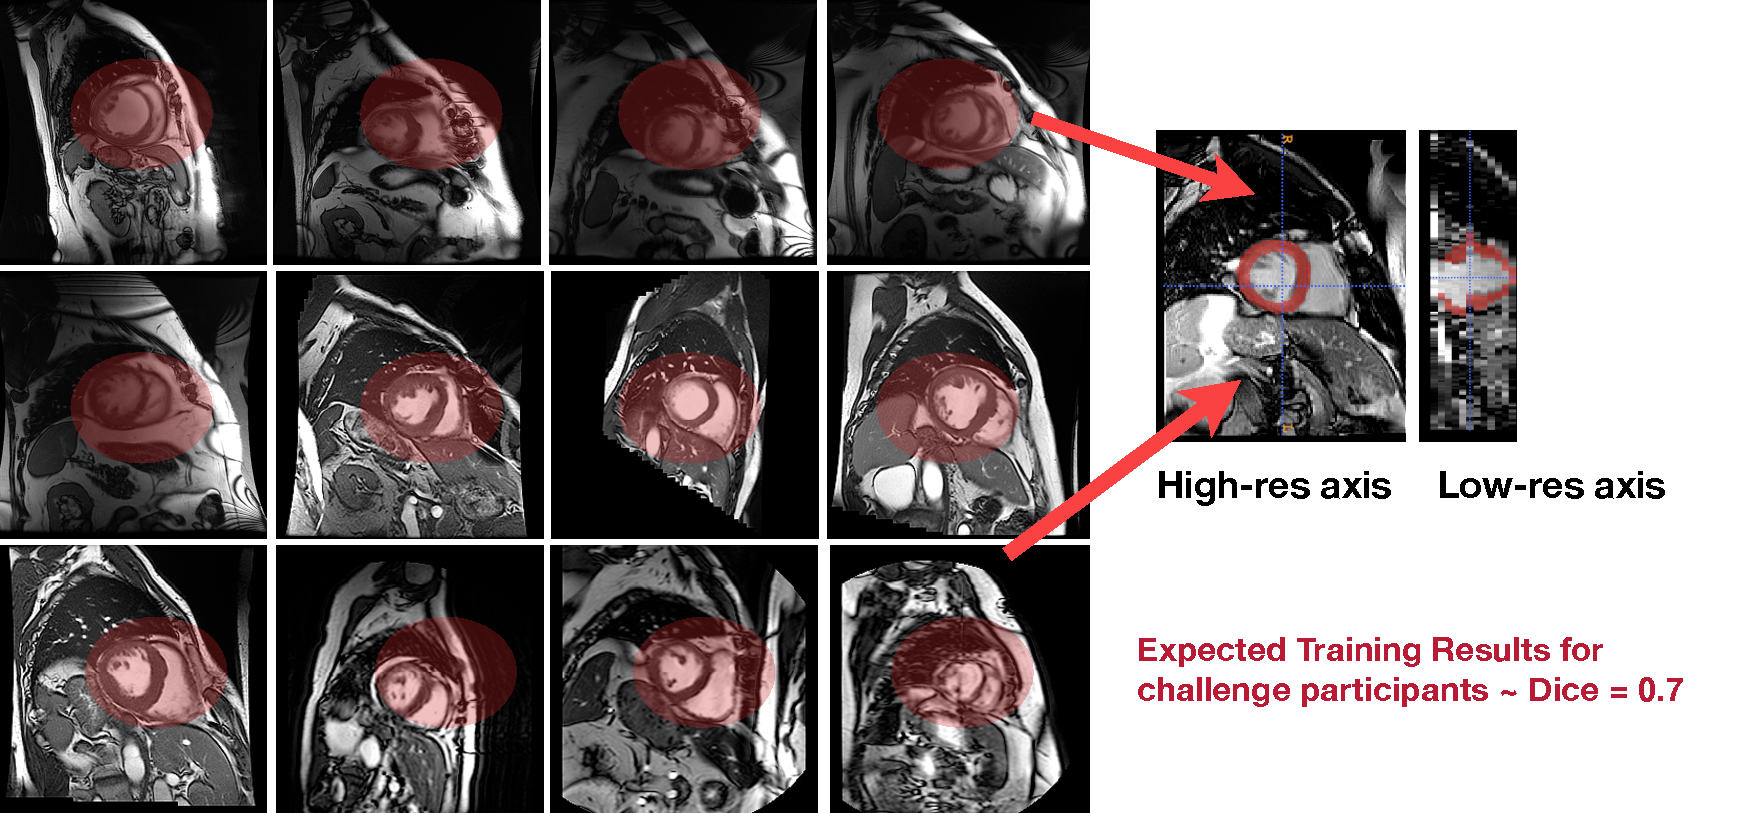
\includegraphics[width=4.5in]{../figs/CAP_methods.pdf}
 \caption{CAP methods focus the registration within a dilated version
of the training image myocardium labeling.  Restricting the
registration focus improves robustness to extra-cardiac features.}
 \label{fig:Cmethods}
\end{figure}

\begin{figure}[t]
 \centering 
  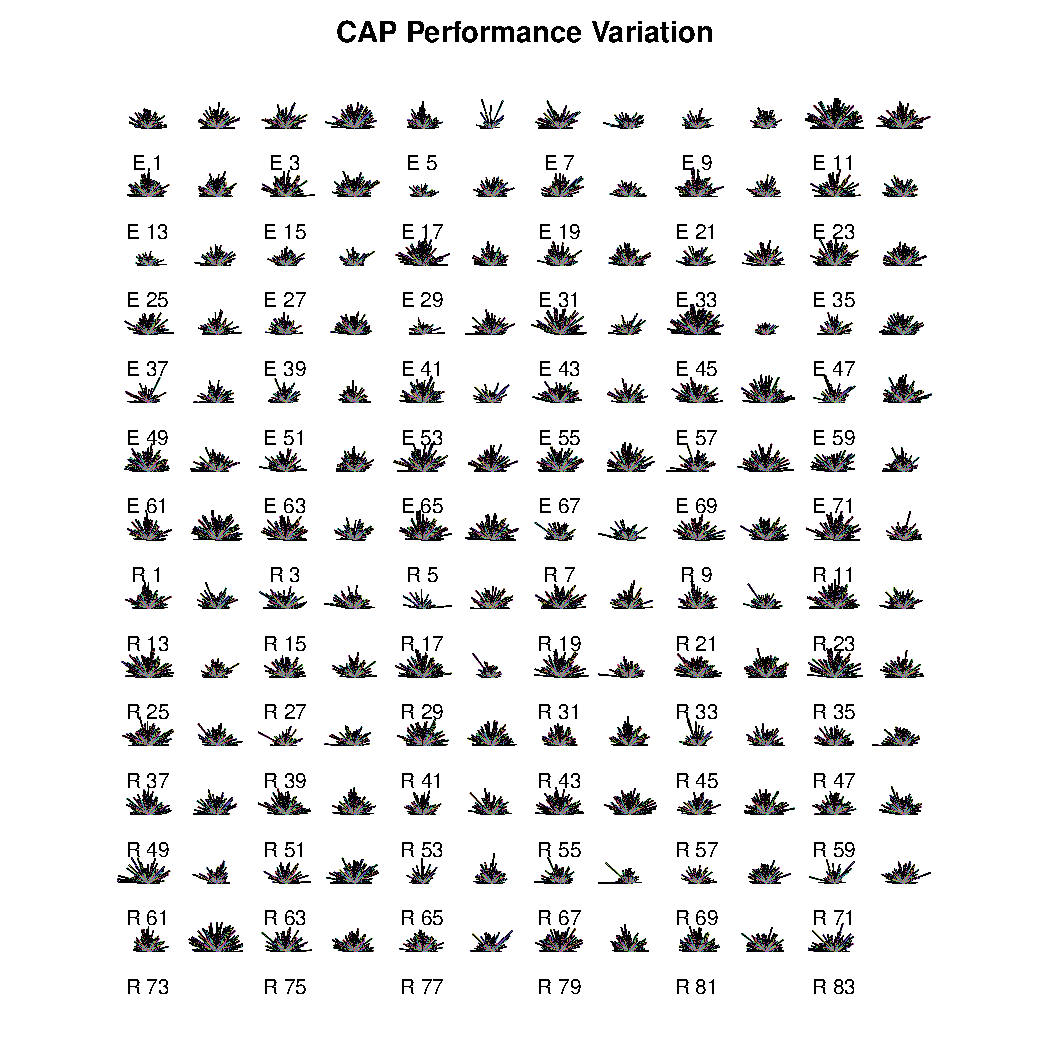
\includegraphics[width=5in]{../figs/spider_CAP.pdf}
 \caption{We use urchin plots to visualize pairwise registration
   performance for CAP data.  We quantified variability in
   all 12,865 data points by measuring
   the global correlation of the deformed image and the target image,
   i.e. both training (labeled R$\star$) and testing (labeled E$\star$). ``Spiky''
   distributions of the correlation function indicate that
 a few pairings performed much better/worse than the majority, at
 least at a global level.  This
 was verified by testing the gaussianity of the resulting correlation
 distribution.  As an example, the sixth subject from top left (E6) has a
 highly non-gaussian distribution of similarity metric performance and
results in a significant p-value for the non-gaussianity test ($p <$
1.e-7 ).  Overall, 13.5\% of subjects exhibited non-gaussian
distributions for this function, after multiple comparisons correction by false discovery rate.}
 \label{fig:CAPvar}
\end{figure}

\section{Discussion} 
The methods described above were informed by experience, the limited
allotted time for processing and the methods available,
contemporaneously, within ANTs, Fire beta.  The ANTs system is
intended to be available to the community such that our results may be
reproduced/extended and improved by the community.  OSX and LINUX are
most actively supported with occasional support for Windows.  The
processing decisions that we made in the standard registration suggest
several possible outcomes and future work, discussed below.  

\subsection{Diencephalon/Brain Data (SATA-B)} The most familiar
problem of the three presented few difficulties.  We did, however,
elect to extract the cerebrum from each image in order to better focus
the results on relevant image features, a strategy that is similar to
that used in the CAP data.  Despite this approach, our pseudo-geodesic
focused on the whole brain should be suboptimal for the diencephalon
data. Entrants that choose to either perform pairwise registration
between all subjects or focus the registration on the diencephalon
should find better performance than the standard approach.  We expect
that entrants should find Dice overlap that is consistent with previous challenges.

\subsection{Dog Leg Multi-Modality Data (SATA-L)}
We employed very little problem-specific optimization for the SATA-L
registration.  It did, however, allow us to test whether two
modalities jointly improve registration results.  Based on a
comparison of single-modality registration and dual modality
registration in the training data, we found the dual modality
similarity metric appeared to increase performance.  We expect that
Dice overlap will be reasonable ($\approx 0.8$ overall as estimated by
H.W.) for the canine leg dataset.

\subsection{CAP Cardiac Data (SATA-C)}
The cardiac dataset reveals some of the limitations involved with
naive pair-wise registration and highlights the benefit of
problem-specific strategies and multi-atlas methods.  We believe that,
of the 3 datasets, the biggest future performance gains may be
possible in this type of data.  Figure~\ref{fig:CAPvar} suggests that,
for some subjects, particular pairings provide a much better matching
than the majority of pairings.  We tested this hypothesis by looking
at the non-gaussianity of the global correlation between the
registered image pairs as calculated within the target subject space.
After FDR-correction, this test suggested that 13.5\% of subjects had
a highly non-gaussian similarity distribution.  For these individuals,
a small portion of training images provide a reasonable result while
the majority might be classified as failures.  This accentuates the
importance of MASR schemes that are robust to high failure rate input
data or the need to cluster the populations before MASR.  While the
organizers requested that the output labels be consistent with the
original 4D manual labels, the intra-rater variability in labeling the
time series is unknown; at first glance, it would seem difficult to
consistently label the myocardium in 3D over several dozen or more
time frames.  Therefore, the upper limits on accuracy remain unclear.
However, we estimated that, with the standard registration, entrants
should achieve up to average Dice overlap of 0.6 to 0.7 as estimated by H.W.  

\section{Conclusions}
Open challenges provide crucial benchmarks to the biomedical image
analysis field and we are honored to play a role in this process.  The
organizers shared excellent challenge data with the community that
should yield exciting results that will advance both
image registration and image segmentation technology.  In particular,
these datasets bring into focus the importance of multiple modality
data, other organ systems and even other species, as well as efficient
registration solutions and the need for MASR methods that are robust
to input data with low reliability.  The SATA data engaged ANTs mean
squared intensity difference, cross-correlation and multivariate
mutual information metrics along with the range of ANTs
transformations, initialization, bias correction and masking options.
We hope that the solutions we provided to the community achieved the
goal set forth: ``provide reasonable \& consistent registration
solutions'' that lead to interesting SATA outcomes.

\bibliographystyle{splncs}
\bibliography{knobsock}
\end{document}



